\chapter{Calibrazione}\label{ch:calibrazione}

% I dati a disposizione
\section{I dati a disposizione}\label{sec:dati}
\ldots

\subsection{Dataset NO2}\label{ssec:dataset-no2}
\ldots

\subsection{Dataset PM2.5 e PM10}\label{ssec:dataset-pm}
\ldots

\subsection{Preprocessamento}\label{ssec:preprocessamento}
\ldots

% Regressione
\section{Regressione}\label{sec:regressione}
Nella statistica applicata come nelle scienze sperimentali si osserva (o si ipotizza) l’esistenza di relazioni fra due o più grandezze.

Sorge allora il problema di determinare una funzione che, in base ai dati ricavati mediante esperimenti o rilevazioni statistiche, rappresenti questi relazioni permettendo, in questo modo, di analizzare meglio i fenomeni osservati.

\subsection{Introduzione}\label{ssec:regressione-introduzione}
Limitando lo studio a problemi che stabiliscono relazioni fra due sole variabili, si tratta, partendo dalle coppie $(x_i, y_i)$ di dati corrispondenti rilevati, di determinare una funzione $y=f(x)$ che rappresenti il fenomeno.

Per trovare una funzione che rappresenti il fenomeno si può procedere in due modi:

\begin{itemize}
  \item determinare una funzione che assuma esattamente i valori $(x_i, y_i)$ rilevati; questo procedimento viene detto interpolazione per punti noti;
  \item determinare una funzione che si accosti il più possibile ai punti $(x_i, y_i)$; questo procedimento viene detto interpolazione fra punti noti.
\end{itemize}

La ricerca di una funzione, generalmente espressa da un polinomio, che passi esattamente per i punti $(x_i, y_i)$ è piuttosto laboriosa; nelle applicazioni statistiche si preferisce determinare una funzione il cui grafico si avvicini ai punti rilevati.

Osservando l’andamento del fenomeno si sceglie il tipo di funzione interpolatrice: lineare, quadratica, esponenziale, ecc. e quindi si procede alla determinazione dei parametri, ossia delle costanti che compaiono nella funzione scelta in modo che sia soddisfatta una condizione di accostamento prefissata.

Per conseguire questo scopo il metodo più utilizzato è il metodo dei \textbf{minimi quadrati} che costituisce un’applicazione della ricerca del minimo di una funzione di più variabili mediante gli strumenti dell’analisi infinitesimale.

Si considerino due variabili $X$ e $Y$ sulle quali si sono effettuate $n$ rilevazioni: $$\left(x_{1}, y_{1}\right),\left(x_{2}, y_{2}\right), \ldots,\left(x_{i}, y_{i}\right), \ldots,\left(x_{n}, y_{n}\right)$$

Sia $y=f(x; a, b, c, ..., k)$ la funzione interpolatrice scelta. Siano inoltre $\hat{y}_{i}$ valori predetti sulla curva corrispondenti ai valori $x_i$ rilevati.

La condizione di accostamento data dal metodo dei minimi quadrati è quella di determinare i valori dei parametri in modo che sia minima la somma dei quadrati delle differenze fra i valori osservati $y_i$ e i valori predetti $\hat{y}_i$ (figura \ref{fig:minimi_quadrati}), ovvero:

$$\varphi(a, b, c, \ldots, k)=\sum_{i=1}^{n}\left[y_{i}-f\left(x_{i} ; a, b, c, \ldots, k\right)\right]^{2}$$\smallskip

dove i valori $x_i$ e $y_i$ sono noti, mentre sono incogniti i parametri $a , b , c , … , k$ della funzione. \cite{excel_per_statistica_belluco}

\begin{figure}[H]
\centering
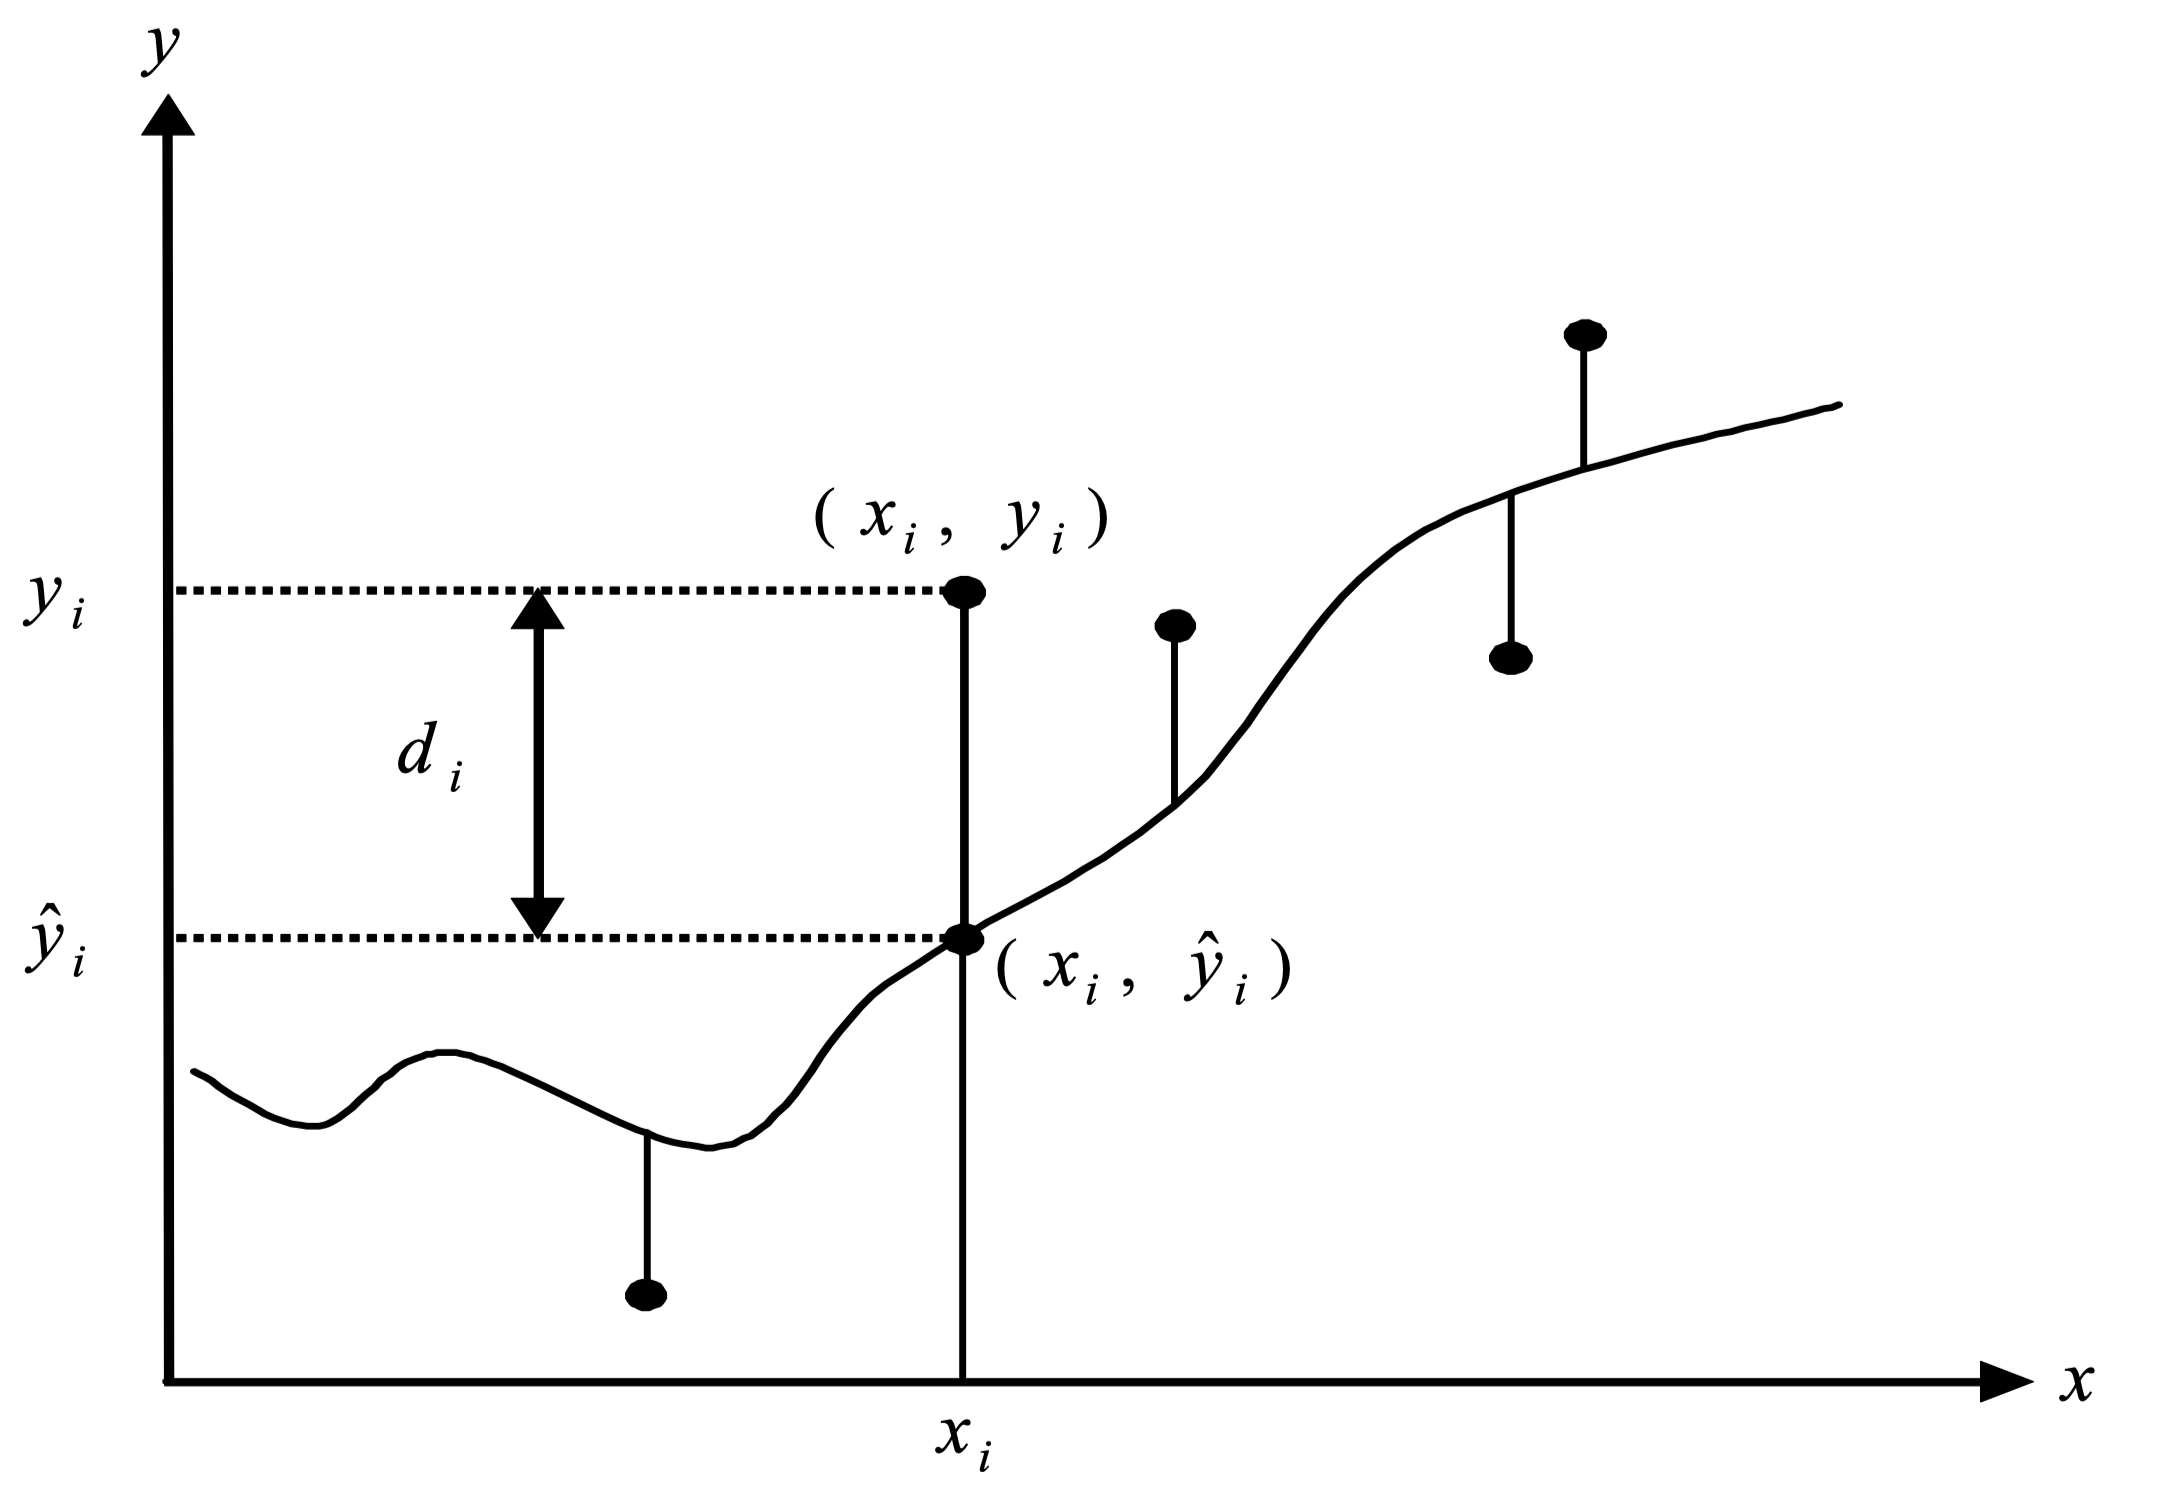
\includegraphics[width=0.75\textwidth,height=\textheight,keepaspectratio]{img/minimi_quadrati.png}
\caption{Condizione dei \textit{minimi quadrati} \cite{excel_per_statistica_belluco}}
\label{fig:minimi_quadrati}
\end{figure}

\subsection{Correlazione e coefficiente di determinazione}\label{ssec:regressione-correlazione}

Quando la dipendenza tra le due variabili è lineare, si parla di correlazione lineare, che può essere valutata mediante il coefficiente di correlazione lineare ($r$):

$$r=\frac{\sum_{i=1}^{n}\left(x_{i}-\bar{x}\right)\left(y_{i}-\bar{y}\right)}{\sqrt{\sum_{i=1}^{n}\left(x_{i}-\bar{x}\right)^{2}} \sqrt{\sum_{i=1}^{n}\left(y_{i}-\bar{y}\right)^{2}}}$$\smallskip

dove il termine al numeratore rappresenta la \textit{covarianza} di $X$ ed $Y$ cioè la variabilità congiunta delle coppie ($x_i$, $y_i$) di valori corrispondenti rispetto al proprio valor medio; mentre il denominatore rappresenta il prodotto delle deviazioni standard di $X$ ed $Y$.

Il coefficiente di correlazione lineare gode di importanti proprietà:

\begin{itemize}
  \item $-1 \le r \le 1$;
  \item si ha $r=1$ quando tutti i dati sono allineati lungo una retta crescente (figura \ref{fig:positive_correlation});
    \begin{figure}[H]
\centering
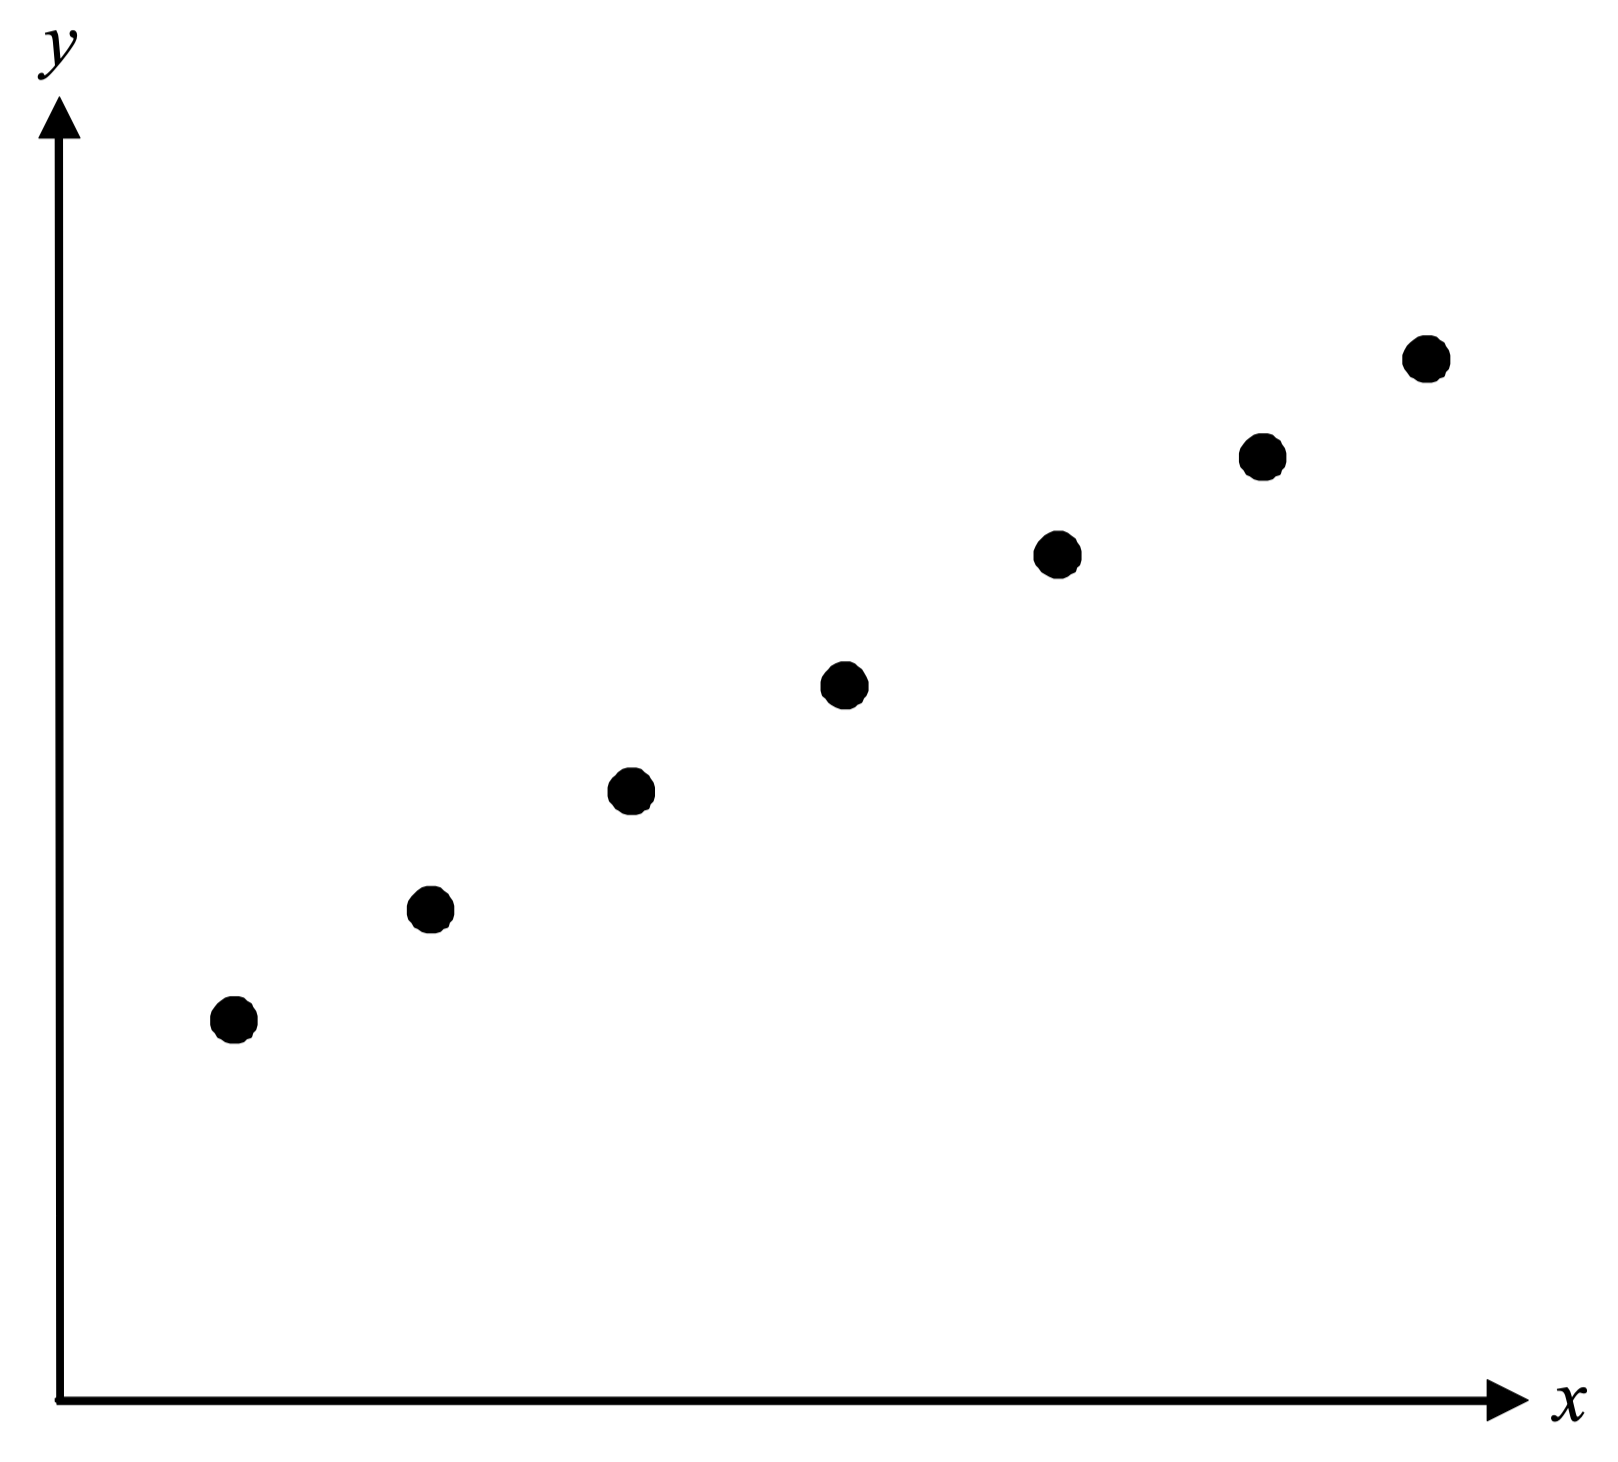
\includegraphics[width=0.55\textwidth,height=\textheight,keepaspectratio]{img/positive_correlation.png}
\caption{Correlazione lineare positiva}
\label{fig:positive_correlation}
\end{figure}

  \item si ha $r=-1$ quando tutti i dati sono allineati lungo una retta decrescente  (figura \ref{fig:negative_correlation});
      \begin{figure}[H]
\centering
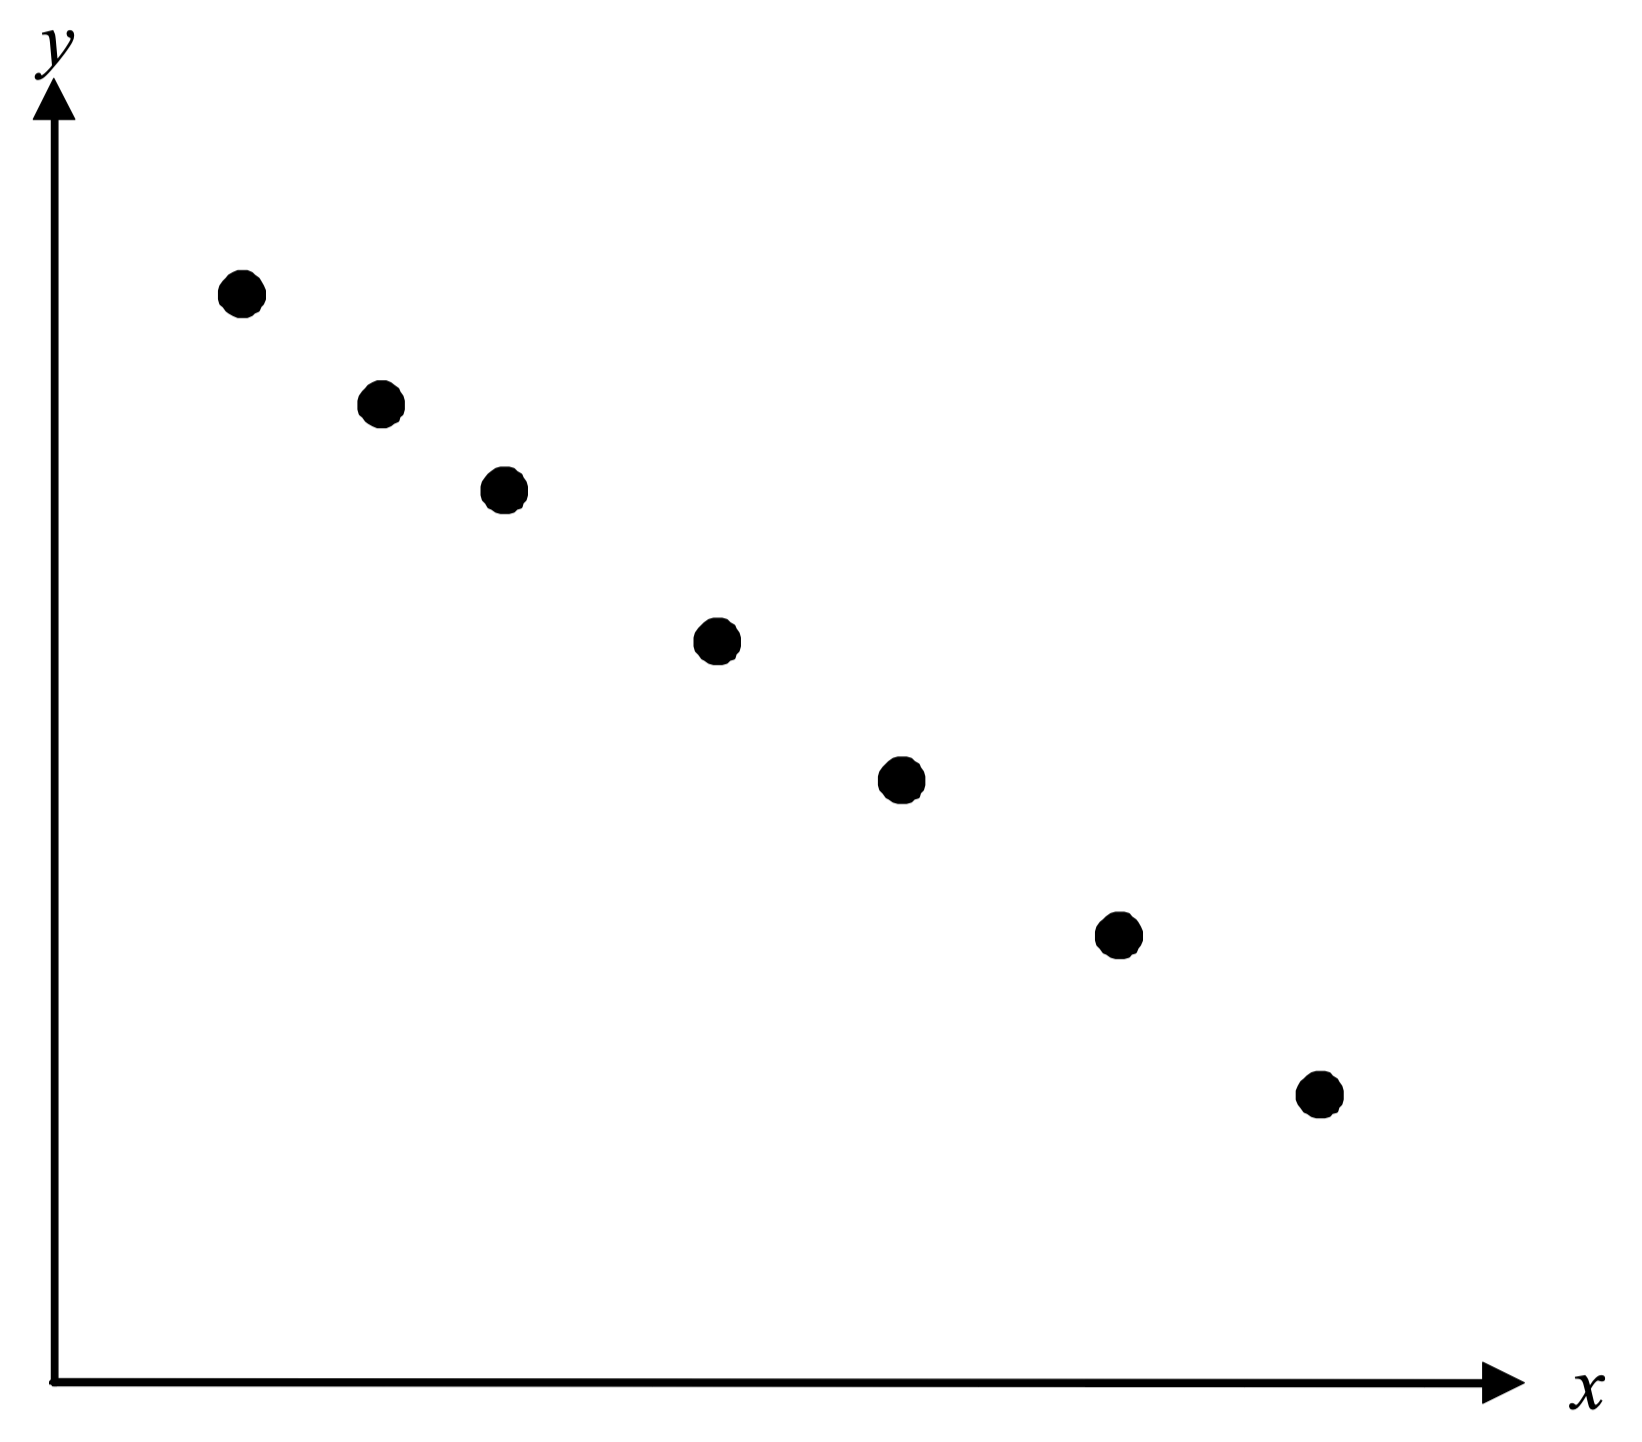
\includegraphics[width=0.55\textwidth,height=\textheight,keepaspectratio]{img/negative_correlation.png}
\caption{Correlazione lineare negativa}
\label{fig:negative_correlation}
\end{figure}
  \item si ha $r=0$ quando non esiste una relazione lineare tra i dati  (figura \ref{fig:no_correlation}).
  \begin{figure}[H]
\centering
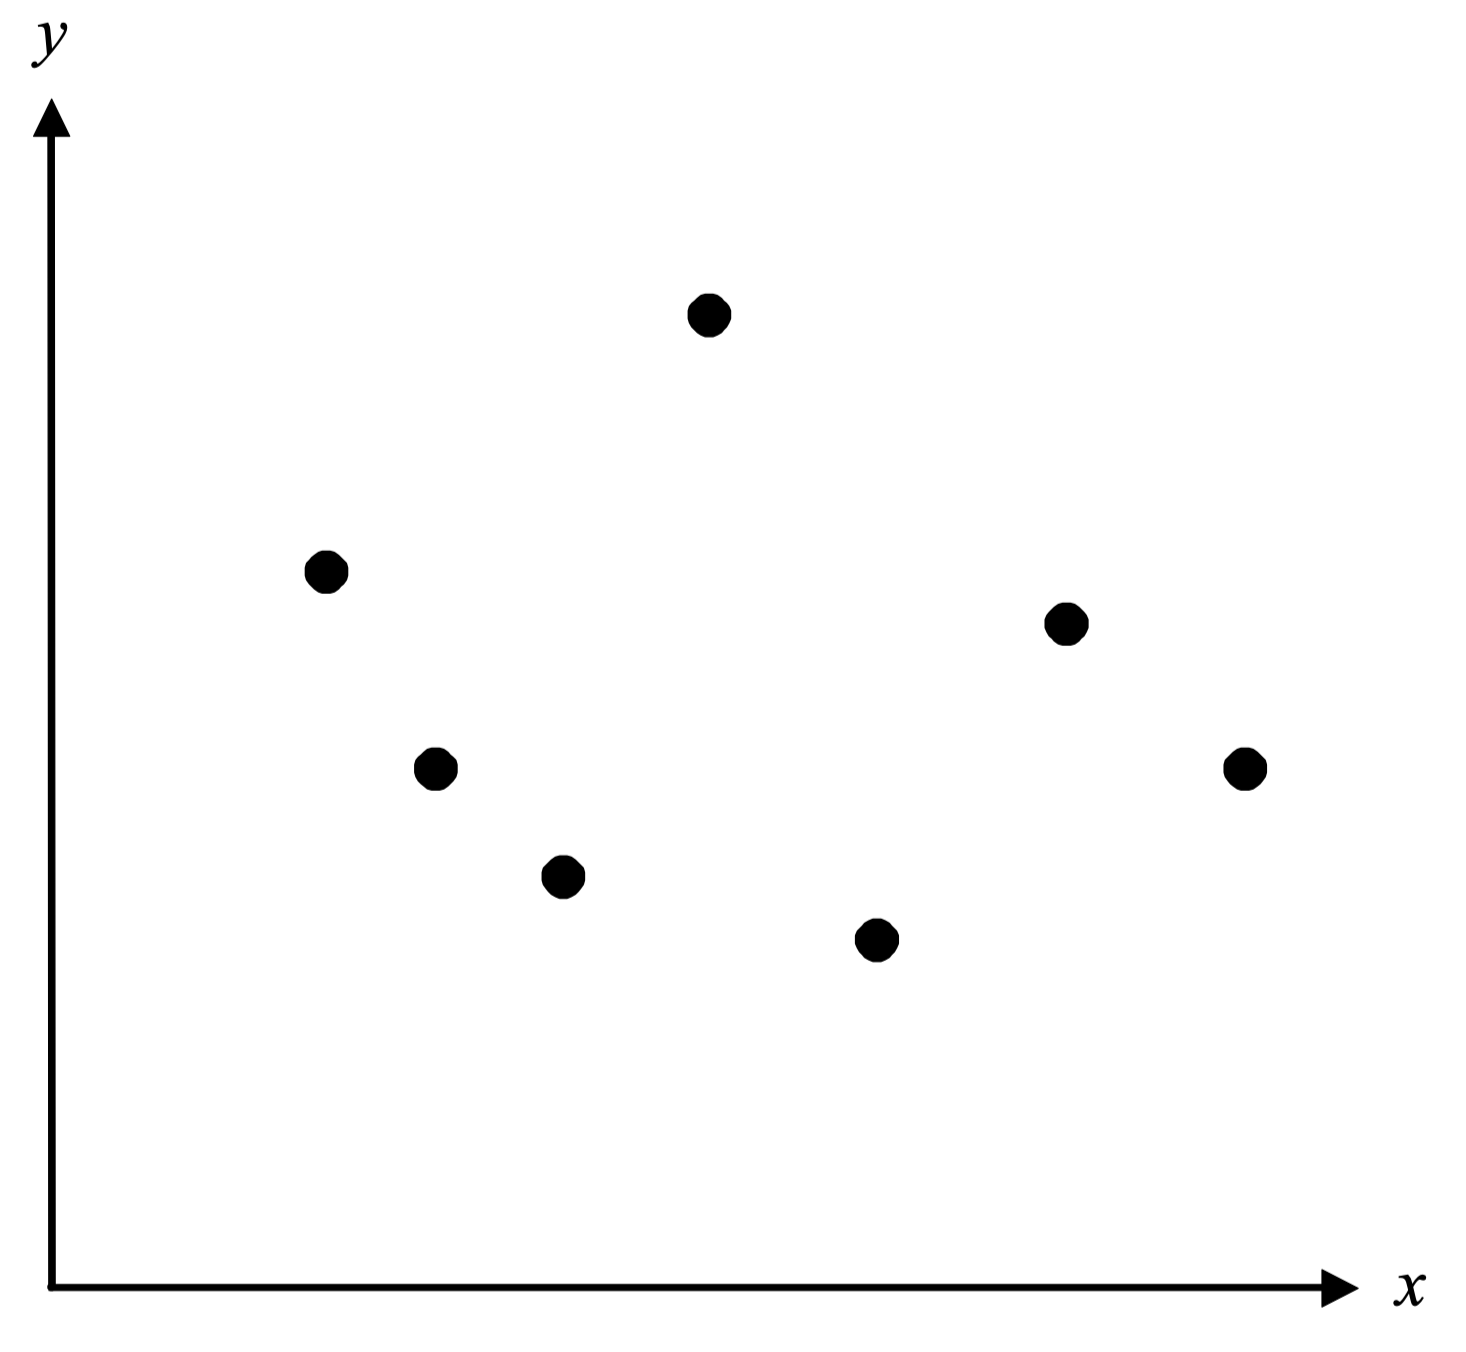
\includegraphics[width=0.55\textwidth,height=\textheight,keepaspectratio]{img/no_correlation.png}
\caption{Nessuna correlazione}
\label{fig:no_correlation}
\end{figure}
\end{itemize}

Sapendo che la varianza ($\sigma_{y}^{2}$) della variabile $Y$ si può scomporre in una parte ($\sigma_{\hat{y}}^{2}$), detta varianza spiegata, in quanto la variabilità della $Y$ è dovuta alla dipendenza di $Y$ dalla variabile $X$, e in una parte ($\sigma_{e}^{2}$), detta varianza non spiegata, in quanto la variabilità della $Y$ non dipende dalla variabile $X$, ma da altri fattori; si può introdurre un secondo indicatore, dato dal rapporto tra la varianza spiegata e la varianza totale, chiamato coefficiente di determinazione:

$$r^{2}=\frac{\sigma_{\hat{y}}^{2}}{\sigma_{y}^{2}}$$\smallskip

che indica quale frazione di varianza totale è dovuta alla dipendenza fra le variabili $Y$ e $X$, ossia quale frazione della variazione della variabile Y è spiegata dalle variazioni della variabile $X$.

Sapendo che:

$$\sigma_{y}^{2}=\sigma_{\hat{y}}^{2}+\sigma_{e}^{2}$$

allora:

$$r^{2}=\frac{\sigma_{\hat{y}}^{2}}{\sigma_{\hat{y}}^{2}+\sigma_{e}^{2}}$$\smallskip

è evidente, quindi, che se la variabilità non spiegata è trascurabile, $\sigma_{e}^{2}$ tende ad annullarsi ed $r^{2}$ avrà un valore prossimo ad 1, mentre diverrà via via minore di 1 al diminuire dell’accordo tra la funzione calcolata e le osservazioni sperimentali.

Minore è la somma residua rispetto alla somma totale dei quadrati, maggiore sarà il valore del coefficiente di determinazione, $r^2$, il quale è un indicatore del livello di precisione con cui l'equazione ottenuta dall'analisi di regressione spiega la relazione tra le variabili. \cite{linear_models}

% TODO aggiungi rmse come metrica

%La regressione è una tecnica statistica che serve a stimare la relazione esistente tra due o più variabili. In particolare, la regressione permette di individuare il coefficiente di correlazione tra due variabili e di determinare se questa relazione è casuale o no.
%
%Tra le applicazioni principali della regressione ci sono:
%
%- Stima della relazione tra due variabili
%
%- Analisi della relazione tra variabili
%
%- Valutazione dell'influenza di una variabile sulle altre
%
%- Predicting

\subsection{Analisi dei residui}\label{ssec:regressione-residui}
Esistono metodi utili per diagnosticare le violazioni delle ipotesi di regressione di base: questi si basano principalmente sullo studio dei residui del modello. Spesso infatti la retta di regressione è infatti una semplificazione della realtà e non coglie tutta la variabilità presente in un insieme di dati. \cite{residui_pozzolo}

Si definiscono i residui come:

$$e_{i}=y_{i}-\hat{y}_{i}, \quad i=1,2, \ldots, n$$\smallskip

dove $y_{i}$ è il valore osservato e $\hat{y}_{i}$ è il valore predetto.

Poiché un residuo può essere visto come la deviazione tra i dati e l'adattamento, è anche una misura della variabilità nella variabile di risposta non spiegata dal modello di regressione. \cite{introduction_to_lr}

Eventuali scostamenti dalle ipotesi sugli errori dovrebbero quindi manifestarsi nei residui. L'analisi grafica dei residui è un modo efficace per scoprire diversi tipi di inadeguatezze del modello, tra cui: 
\begin{itemize}
  \item se i residui hanno distribuzione normale (\ref{ssec:distr-errori});
  \item se le varibabili indipendenti sono correlate con l'errore (\ref{ssec:correlazione-errore-variabili});
  \item se la varianza dei residui è omogenea (\ref{ssec:omogeneita-varianza});
  \item se ci sono degli outliers che influenzano la pendenza della retta (\ref{ssec:influenza-outliers}).
\end{itemize}

\subsubsection{Distribuzione degli errori}\label{ssec:distr-errori}
La distribuzione normale degli errori può essere verificata attraverso un grafico dei quantili, detto anche q-q plot.
In questa tipologia di grafico, i quantili teorici di una distribuzione Normale sono riportati sull’asse orizzontale. I quantili dei residui standardizzati sono invece riportati sull’asse verticale.
L’idea è che se i residui hanno una distribuzione normale, i loro quantili dovrebbero coincidere con quelli della distribuzione normale. A livello visivo, questo significa che i punti dovrebbero disporsi lungo la \textit{bisettrice}, indicata dalla retta presente nel grafico (figura TODO).

%TODO figura + ref

Nella pratica, non capita quasi mai che i punti si dispongano esattamente lungo la bisettrice. Per poter dire che gli errori hanno una distribuzione normale ci si accontenta quindi che i punti siano vicino alla linea presente nel grafico.
Tuttavia in generale le stime sui coefficienti di regressione sono abbastanza robuste a violazioni della normalità distributiva dei residui.

\subsubsection{Correlazione tra errore e variabili}\label{ssec:correlazione-errore-variabili}
Se una variabile esplicativa è correlata con il termine d’errore, è possibile utilizzare questa variabile esplicativa per predire quale sarà l’errore del modello di regressione. Questo in generale non è un buon segno, perché la componente di errore di un modello di previsione deve essere imprevedibile.

Per verificare la non correlazione tra la variabile indipendente (x) e i residui è utile osservare un grafico di dispersione come quello riportato in figura TODO, in sull’asse orizzontale si mettono i valori della x, mentre sull’asse verticale i valori dei residui.

%TODO figura + ref

L’ipotesi è confermata se non è individuabile nessuna relazione tra le due variabili.

\subsubsection{Omogeneità della varianza dei residui}\label{ssec:omogeneita-varianza}
Per verificare l’ipotesi di omogeneità delle varianze dei residui, è necessario creare un grafico a dispersione.  I valori stimati della y si riportano sull’asse orizzontale delle x. Sull’asse verticale delle y invece si indicano i valori dei residui (figura \ref{fig:distr_residui}).

\begin{figure}[H]
\centering
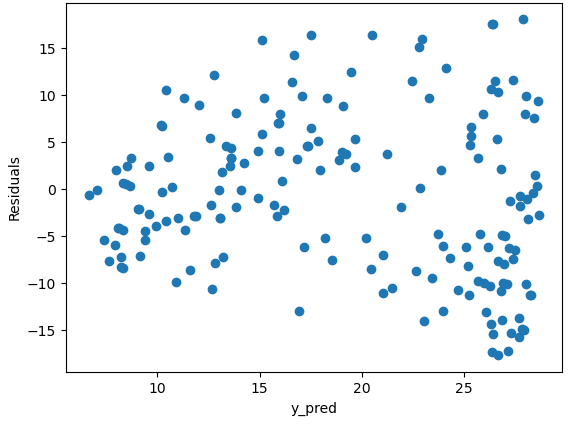
\includegraphics[width=0.65\textwidth,height=\textheight,keepaspectratio]{img/distr_residui.png}
\caption{Esempio di distribuzione dei residui}
\label{fig:distr_residui}
\end{figure}

Se c’è omogeneità della varianza dei residui, i punti saranno dispersi in modo simile sia nella parte sinistra che in quella destra del grafico. Questa proprietà se verificata prende il nome di \textbf{omoschedasticità}.

\subsubsection{Influenza di outliers}\label{ssec:influenza-outliers}
Il grafico a dispersione tra valori predetti e residui permette di individuare anche i possibili outliers, ovvero i punti isolati nel grafico (quelli con residui maggiori).
Tuttavia, per verificare se ci sono outliers in un modello di regressione, spesso si utilizzano altre tecniche (ad esempio eliminando i punti problematici tramite la distanza di Cook, descritta in \ref{sssec:regressione-cook}, oppure applicando stime robuste meno sensibili alle le osservazioni problematiche, ad esempio con la funzione peso di Huber  descritta in \ref{sssec:regressione-huber}). Nel primo caso è utile anche provare a rifare le analisi di regressione escludendo le osservazioni potenzialmente problematiche e vedere se ci sono differenze nei coefficienti del modello.

Nei modelli di regressione infatti anche un singolo outlier può influenzare in maniera sostanziale la capacità di adattamento del modello ai dati, soprattutto se il campione non è molto numeroso.

\subsection{Modelli di regressione}\label{ssec:regressione-modelli}
I modelli di regressione sono ampiamente utilizzati sia per la previsione o la descrizione dei dati che la stima e il controllo dei parametri.

\subsubsection{Regressione lineare}\label{sssec:regressione-lineare}
Si considera una funzione lineare a due variabili:
$$y = a + b*x$$

In questo caso si deve rendere minima la funzione:

$$\varphi(a, b)=\sum_{i=1}^{n}\left[y_{i}-\left(a+b x_{i}\right)\right]^{2}$$\smallskip

Annullando le derivate parziali prime rispetto ad $a$ e $b$ si ha il sistema:

$$\left\{\begin{array}{l}
\sum_{i=1}^{n} 2\left[y_{i}-\left(a+b x_{i}\right)\right](-1)=0 \\
\sum_{i=1}^{n} 2\left[y_{i}-\left(a+b x_{i}\right)\right]\left(-x_{i}\right)=0
\end{array}\right.$$\smallskip

che risolto, fornisce i valori dei parametri:

$$\left\{\begin{array}{l}
\hat{a}=\bar{y}-b \bar{x} \\
\hat{b}=\frac{\sum_{i=1}^{n}\left(x_{i}-\bar{x}\right)\left(y_{i}-\bar{y}\right)}{\sum_{i=1}^{n}\left(x_{i}-\bar{x}\right)^{2}}
\end{array}\right.$$\smallskip

dove $\bar{x}$ e $\bar{y}$ indicano le \textit{medie aritmetiche}, rispettivamente di $x_i$ e $y_i$.

La stima del parametro $b$, \textit{coefficiente angolare} della funzione lineare, può essere rappresentato nella forma:

$$\hat{b}=\frac{\sum_{i=1}^{n} \frac{\left(x_{i}-\bar{x}\right)\left(y_{i}-\bar{y}\right)}{n}}{\sum_{i=1}^{n} \frac{\left(x_{i}-\bar{x}\right)^{2}}{n}}$$\smallskip

dove il denominatore è la \textit{varianza} di $X$ ($\sigma_{X}^{2}$), mentre il numeratore è detto \textit{covarianza} di X e Y ($\sigma_{XY}$) e misura la variabilità congiunta delle coppie ($x_i$, $y_i$) di valori corrispondenti rispetto al proprio valor medio; quindi, il coefficiente $b$ della retta interpolante esprime la variabilità congiunta di $X$ e $Y$ rapportata alla variabilità della sola $X$.

\begin{figure}[H]
\centering
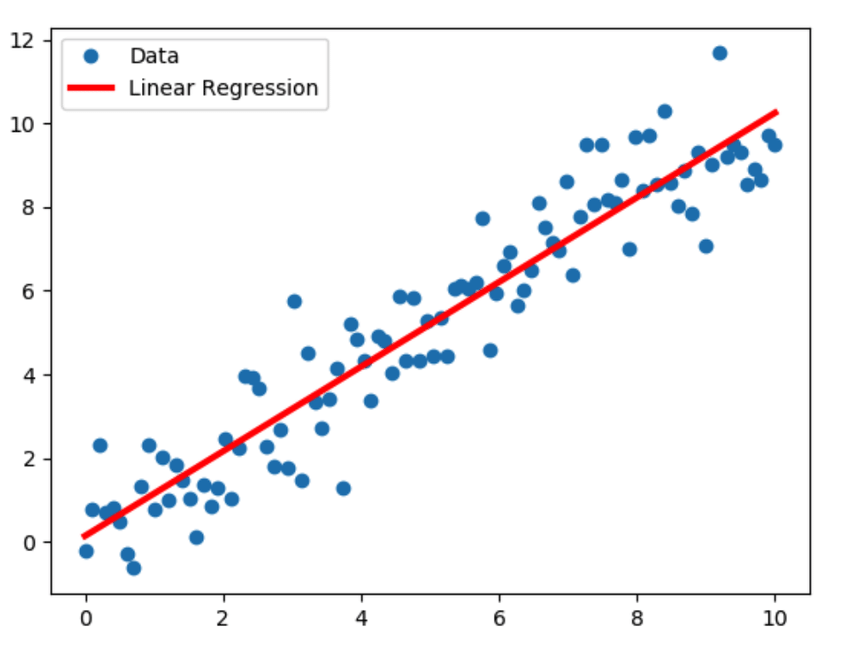
\includegraphics[width=0.65\textwidth,height=\textheight,keepaspectratio]{img/lin_reg_example.png}
\caption{Esempio di regressione lineare}
\label{fig:reg_lin}
\end{figure}

La precisione della retta calcolata dalla regressione lineare dipende dal grado di dispersione nei dati. Più i dati sono lineari, più il modello risulterà accurato.

%Per stimare la relazione tra due variabili, la regressione lineare utilizza una formula matematica che calcola la media dei valori della prima variabile (Y) in funzione dei valori della seconda variabile (X). La formula della regressione lineare è:
%
%Y = a + bX
%
%In questa formula, a è la costante di regressione e b è la coefficiente di regressione. La costante di regressione a indica la media dei valori di Y in funzione dei valori di X. Il coefficiente di regressione b indica la relazione tra le due variabili: più è vicino a 1, più le due variabili sono correlate in modo lineare.
%
%Utilizzando la regressione lineare, è possibile stimare la relazione tra due variabili anche in presenza di deviazioni dalla linea.

\subsubsection{Regressione lineare robusta (Huber)}\label{sssec:regressione-huber}
La regressione Huber (in inglese Huber regression, anche detta regressione robusta) è una metodologia statistica per la stima dei parametri di un modello lineare in presenza di \textit{outliers}.

Ci sono situazioni in cui si verifica presenza di valori anomali che influiscono sul modello di regressione, nel senso che possono avere una forte influenza sul metodo dei minimi quadrati, di fatto \textit{deviando} troppo l'equazione di regressione nella loro direzione. Il metodo dei minimi quadrati, infatti, in questi casi ha lo svantaggio di avere la tenedenza a essere dominato da questi valori — infatti sommando il quadrato dei residui ($\sum_{i=1}^{n} a_i^2$ dove $a_i$ è il residuo i-esimo), la media risulta troppo influenzata da pochi valori $a_i$ particolarmente grandi.

Ci sono due modi per affrontare questa situazione:

\begin{itemize}
  \item Scartare le osservazioni \textit{scomode} (vedi regressione lineare avanzata \ref{sssec:regressione-cook});
  \item Applicare procedure di stime robuste in modo che siano meno sensibili alle osservazioni troppo influenti (figura \ref{fig:reg_rob}).
\end{itemize}

\begin{figure}[H]
\centering
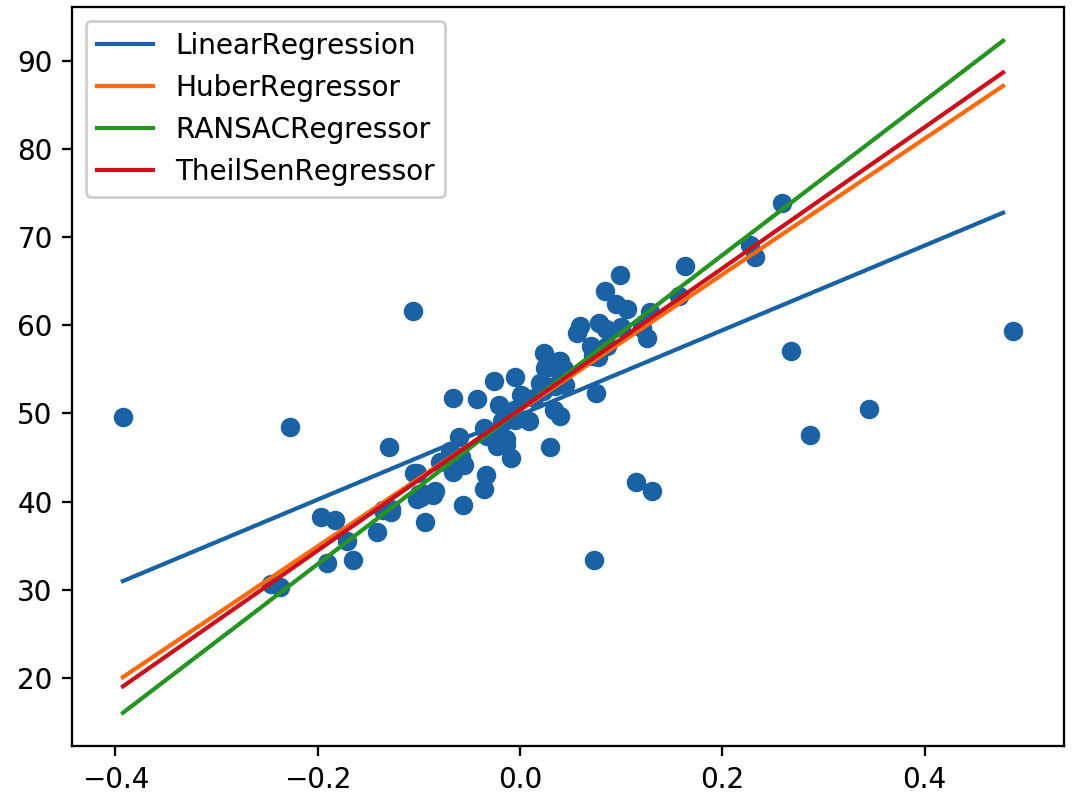
\includegraphics[width=0.65\textwidth,height=\textheight,keepaspectratio]{img/robust.png}
\caption{Comportamento di modelli di regressione robusta in presenza di outliers}
\label{fig:reg_rob}
\end{figure}

Una delle funzioni di stima robusta, comunemente usata in diversi metodi di regressione per ridurre la sensibilità dei parametri alla presenza di outliers, è la \textbf{funzione di Huber}, che risulta quadratica per piccoli valori di $x$, e lineare per valori più grandi. È definita come:

$$L_{\delta}(a)= \begin{cases}\frac{1}{2} a^{2} & \text { per }|a| \leq \delta \\ \delta\left(|a|-\frac{1}{2} \delta\right), & \text { altrimenti }\end{cases}$$\smallskip

Dove la variabile $a$ fa riferimento al residuo, cioè la differenza tra valore osservato e valore predetto ($a = y - f(x)$).


\subsubsection{Regressione lineare avanzata}\label{sssec:regressione-cook}
Come accennato in \ref{sssec:regressione-huber}, un'altra tecnica per la gestione di outlier è quella di applicare il modello sul dataset dopo aver rimosso i valori anomali. Esistono molte metriche su cui basarsi per rimuovere gli outlier da un set di dati: un metodo che viene spesso utilizzato nella regressione è la \textbf{distanza di Cook}.

La distanza di Cook è una stima dell'\textit{influenza} di una osservazione in un dataset, in termini di residuo (outlier) o di elevato \textit{leverage}: è un riepilogo di quanto cambierebbe un modello di regressione nel caso in cui venga rimossa l'i-esima osservazione.

In presenza di outliers la distanza di Cook aumenta, e quindi questi dati ad alta influenza hanno un maggiore impatto sulle stime dei parametri della regressione.

La distanza di Cook \cite{cook_def} dell'osservazione $i$ ($\forall i=1, \ldots, n$) è definita come:

$$D_{i}=\frac{\sum_{j=1}^{n}\left(\hat{y}_{j}-\hat{y}_{j(i)}\right)^{2}}{p s^{2}}$$\smallskip

dove:

\begin{itemize}
  \item $n$ è il numero di osservazioni;
  \item $\hat{y}_{j}$ è il valore predetto;
  \item $\hat{y}_{j(i)}$ è la risposta ottenuta escludendo l'i-esima osservazione.
\end{itemize}

Oppure, in modo equivalente:

$$D_{i}=\frac{e_{i}^2}{p s^{2}}\left[\frac{h_{i}}{\left(1-h_{i}\right)^{2}}\right]$$\smallskip

dove:

\begin{itemize}
  \item $e_{i} = y_i - \hat{y_i}$  è l'i-esimo residuo;
  \item $p$ è il numero di coefficienti della regressione;
  \item $s^2$ è l'errore quadratico medio (MSE);
  \item $h_i$ è il peso che l'i-esimo osservazione ha sul valore della regressione (\textit{leverage}).
\end{itemize}

Un esempio di rilevazione grafica di outlier tramite distanza di Cook è riportato in figura \ref{fig:cook}.

\begin{figure}[H]
\centering
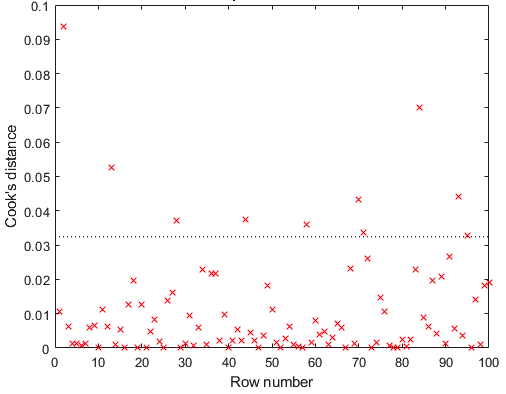
\includegraphics[width=0.65\textwidth,height=\textheight,keepaspectratio]{img/cook.png}
\caption{Riconoscimento di outlier tramite distanza di Cook}
\label{fig:cook}
\end{figure}

Vi sono diverse opinioni riguardo al valore di soglia di \textit{cut-off}, oltre la quale un dato può essere considerato un outlier. In \cite{applied_regression} viene proposta:

$$D_{i}>\frac{4}{n}$$\smallskip

dove $n$ è il numero di osservazioni. La distanza di Cook può anche essere utilizzata per individuare regioni dello spazio nelle quali sarebbe necessario effettuare una validazione, ad esempio acquisendo più dati.

\subsubsection{Regressione Ridge}\label{sssec:regressione-ridge}
Nella statistica e nel Machine Learning, la regressione Ridge è un metodo di analisi di regressione che applica una fase di \textbf{regolarizzazione} al fine di migliorare l'accuratezza della previsione, prevenire l'\textit{overfitting} e penalizzare la complessità del modello.
Insieme al LASSO (vedi \ref{sssec:regressione-lasso}) è un modello di regressione che viene ripreso anche da tecniche di Boosting di Machine Learning.

Parlando di regolarizzazione in generale esistono due tipi di penalizzazione:
\begin{itemize}
  \item \textbf{L1}: penalizza il valore assoluto dei coefficienti del modello (es. Lasso); 
  \item \textbf{L2}: penalizza il quadrato del valore dei coefficienti del modello (es. Ridge).
\end{itemize}

La regressione Ridge usa la penalità L2: in pratica questo produce coefficienti piccoli, ma nessuno di loro è mai annullato (\textit{feature shrinkage}).

Richiamando il metodo dei minimi quadrati (\ref{ssec:regressione-introduzione}) si deve minimizzare la somma dei quadrati dei residui (RSS):

$$\mathrm{RSS}=\sum_{i=1}^{n}\left(y_{i}-\beta_{0}-\sum_{j=1}^{p} \beta_{j} x_{i j}\right)^{2}$$\smallskip

Nella regressione Ridge si aggiunge anche un termine di penalità, ottenendo quindi:

$$\sum_{i=1}^{n}\left(y_{i}-\beta_{0}-\sum_{j=1}^{p} \beta_{j} x_{i j}\right)^{2}+\lambda \sum_{j=1}^{p} \beta_{j}^{2}=R S S+\lambda \sum_{j=1}^{p} \beta_{j}^{2}$$\smallskip

Dove $\lambda$ è un parametro di \textit{tuning} che serve proprio a controllare l’effetto della penalità: un valore $\lambda=0$ infatti non avrà effetto sul risultato finale (l’equazione viene ricondotta a quella dei minimi quadrati), al contrario per $\lambda \to \infty$ invece i coefficienti di regressione stimati tenderanno a zero poiché si darà molto peso alla penalità del modello. \cite{lasso_vs_ridge}

Il modello di Ridge Regression presenta dei vantaggi rispetto a quello dei minimi quadrati, soprattutto per quanto riguarda il \textit{bias-variance trade-off}: in generale, quando c’è una relazione lineare tra i predittori e la variabile risposta, il modello dei minimi quadrati comporta poco bias ma alta varianza. Questo si traduce nel fatto che una piccola variazione nel training data può generare un cambiamento notevole nei coefficienti stimati; di contro la Ridge regressione lavora bene nelle situazioni dove il modello dei minimi quadrati genera ampia varianza nelle stime.\cite{tesi_polito}

\subsubsection{Regressione Lasso}\label{sssec:regressione-lasso}
Lo svantaggio della regressione Ridge è il fatto di considerare tutte le variabili per la predizione nel modello finale. Il termine di regolarizzazione $\lambda \sum_{j=1}^{p} \beta_{j}^{2}$ tende ad assegnare ai coefficienti valori vicini allo zero, ma non perfettamente zero, a meno che $\lambda = 0$.
Questo non crea problemi per l’ accuratezza della predizione quanto per l’interpretazione delle varabili, soprattutto quando il numero delle variabili diventa alto.

La regressione Lasso (acronimo di \textit{least absolute shrinkage and selection operator}, ovvero operatore di restringimento e selezione minimo assoluto) è un’alternativa alla regressione ridge utilizzata proprio per superare questo problema. L'unica differenza sta nel termine di regolarizzazione, ovvero:

$$\lambda \sum_{j=1}^{p}\left|\beta_{j}\right|$$\smallskip

Per cui l'equazione del modello diventa:

$$\sum_{i=1}^{n}\left(y_{i}-\beta_{0}-\sum_{j=1}^{p} \beta_{j} x_{i j}\right)^{2}+\lambda \sum_{j=1}^{p}\left|\beta_{j}\right|=R S S+\lambda \sum_{j=1}^{p}\left|\beta_{j}\right|$$\smallskip

Anche nel caso di Lasso regression il parametro di regolarizzazione tende a stimare i valori dei coefficienti verso lo zero ma, a differenza della regressione ridge, la penalità $\lambda \sum_{j=1}^{p}\left|\beta_{j}\right|$ costringe uno o più coefficienti ad essere esattamente zero per certi valori di $\lambda$. \cite{tesi_polito}

\subsubsection{Regressione polinomiale}\label{sssec:regressione-polinomiale}
La regressione polinomiale è una generalizzazione della regressione lineare, infatti utilizza lo stesso metodo matematico della variante lineare, ma assume che la relazione di funzione che caratterizza i dati sia meglio descritta, anzichè da una retta, da un polinomio. In questo caso il metodo dei minimi quadrati può essere utilizzato anche per adattare una funzione polinomiale a un insieme di dati. Considerato un polinomio di grado $k$:

$$y=a_{0}+a_{1} x+a_{2} x^{2}+a_{3} x^{3}+\ldots+a_{k} x^{k}$$\smallskip

In questo caso il sistema di equazioni da risolvere è:

$$\left\{\begin{array}{l}
n a_{0}+a_{1} \sum_{i=1}^{n} x_{i}+a_{2} \sum_{i=1}^{n} x_{i}^{2}+\cdots+a_{k} \sum_{i=1}^{n} x_{i}^{k}=\sum_{i=1}^{n} y_{i} \\
a_{1} \sum_{i=1}^{n} x_{i}+a_{2} \sum_{i=1}^{n} x_{i}^{2}+\cdots+a_{k} \sum_{i=1}^{n} x_{i}^{k}=\sum_{i=1}^{n} x_{i} y_{i} \\
\cdots \\
a_{1} \sum_{i=1}^{n} x_{i}^{k}+a_{2} \sum_{i=1}^{n} x_{i}^{k+1}+\cdots+a_{k} \sum_{i=1}^{n} x_{i}^{2 k}=\sum_{i=1}^{n} x_{i}^{k} y_{i}
\end{array}\right.$$\smallskip

che, risolto, permette di ricavare i parametri $a_0$, $a_1$, $a_2$, ..., $a_k$.

I polinomi sono ampiamente utilizzati in situazioni in cui la risposta è curvilinea, poiché anche relazioni non lineari complesse possono essere adeguatamente modellate da polinomi su intervalli ragionevolmente piccoli delle $x$.

\begin{figure}[H]
\centering
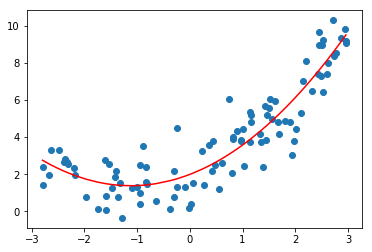
\includegraphics[width=0.65\textwidth,height=\textheight,keepaspectratio]{img/poly_reg_example.png}
\caption{Esempio di regressione polinomiale}
\label{fig:poly_reg}
\end{figure}

Ci sono diverse considerazioni importanti che emergono quando si adatta un polinomio in una variabile: una di queste riguarda la scelta dell'ordine del modello.
Come regola generale, l'uso di polinomi di ordine elevato ($k > 2$) dovrebbe essere evitato: un modello di ordine basso è quasi sempre preferibile a un modello di ordine elevato per ragioni di minore complessità, di coerenza con i dati e per evitare \textit{overfitting}.

Come caso estremo, è sempre possibile trovare un polinomio di grado $n-1$ ad $n$ punti che risulti in un buon adattamento dei dati.
Nella maggior parte dei casi, però, questo non farebbe nulla per migliorare la comprensione della funzione sconosciuta, né sarà probabilmente un buon predittore.

\subsubsection{Regressione con Random Forest}\label{sssec:regressione-rf}
La regressione Random Forest è un algoritmo di apprendimento supervisionato che utilizza il metodo di apprendimento \textit{ensemble} per la regressione tramite alberi di decisione. Il metodo di apprendimento ensemble è una tecnica che combina le previsioni di più algoritmi di apprendimento automatico per effettuare una previsione più accurata rispetto a un singolo modello. \cite{random_forest}

In particolare, una foresta casuale (random forest) opera adattando una serie di alberi decisionali su vari sottocampioni del set di dati e utilizza la media dei risultati per migliorare l'accuratezza predittiva e controllare l'overfitting.
In breve, l'algoritmo funziona esegue i seguenti passi:

\begin{enumerate}
  \item Sceglie a caso $k$ osservazioni dati dal training set;
  \item Costruisce un albero decisionale associato a queste $k$ osservazioni;
  \item Sceglie il numero $N$ di alberi da costruire e ripete i passaggi 1 e 2 per ciascuno;
  \item Per una nuova osservazione, fa in modo che ciascuno degli $N$ alberi preveda il valore di $y$, e assegna il nuovo punto alla media su tutti i valori $y$ previsti.
\end{enumerate}

Uno dei principali svantaggi degli alberi decisionali è che sono molto inclini a fare \textit{overfitting}: funzionano bene sui dati di training, ma non sono così flessibili per fare previsioni su campioni invisibili. Sebbene ci siano soluzioni alternative per questo, come ad esempio ridurre gli alberi, questo riduce il loro potere predittivo. Generalmente sono modelli con bias medio e varianza alta, ma sono semplici e di facile interpretazione.

\subsubsection{Regressione con Gradient Boosting}\label{sssec:regressione-gb}
Il Gradient Boosting è una tecnica di Machine Learning che ha alla base la stima iterativa di alberi sui residui ottenuti ad ogni passo e l’aggiornamento in maniera adattiva delle stime. Questa tecnica riprende il concetto matematico del \textit{Gradient Descent}, per cui lo split scelto sarà quello che favorisce l’avvicinamento al punto di minimo della funzione obiettivo.

Il Gradient Descent è un algoritmo di ottimizzazione che consente di individuare il valore minimo di una funzione di costo per sviluppare un modello con una previsione accurata.

L’algoritmo Gradient Boosting applicato a problemi di regressione può essere descritto nei seguenti passi:

\begin{enumerate}
  \item Si inizializza il modello con un valore noto;
  \item Si considera sul training set una \textit{loss function}, ovvero una funzione differenziabile che esprima una valutazione della predizione (es. $\frac{1}{2} (y_i - \hat{y}_{i})$ dove $y_i$ è l'osservazione e $\hat{y}_{i}$ è la predizione);
  \item Scelto il numero massimo di alberi, per ciascuno si modella un albero di regressione seguendo na procedura di discesa del gradiente in modo da minimizzare la perdita. L'albero ottenuto viene aggiunto alla sequenza di alberi già esistente, nel tentativo di correggere o migliorare l'output finale del modello.
\end{enumerate}


\subsubsection{Regressione con SVR}\label{sssec:regressione-svr}
\ldots

\subsubsection{Regressione con KernelRidge}\label{sssec:regressione-kridge}
\ldots
% TODO cita libro che c'è in fondo a https://scikit-learn.org/stable/modules/kernel_ridge.html#id1

% Esperimenti e risultati ottenuti
\section{Esperimenti e risultati ottenuti}\label{sec:esperimenti}
\ldots

\subsection{NO2}\label{ssec:risultati-no2}
\ldots

\subsection{PM2.5}\label{ssec:risultati-pm2.5}
\ldots

\subsection{PM10}\label{ssec:risultati-pm10}
\ldots

% Validazione
\section{Validazione}\label{sec:validazione}
%TODO vedi capitolo 11 di douglas
%TODO vedi anche https://en.wikipedia.org/wiki/Regression_validation

Poiché l'adattamento del modello ai dati disponibili costituisce la base per molte delle tecniche utilizzate nel processo di sviluppo del modello (come la selezione delle variabili), si è tentati di concludere che un modello che si adatta bene ai dati avrà successo anche nel applicazione finale. Non é necessariamente così. Ad esempio, un modello potrebbe essere stato sviluppato principalmente per prevedere nuove osservazioni.

Non vi è alcuna garanzia che l'equazione che fornisce il miglior adattamento ai dati esistenti sarà un predittore di successo. Fattori influenti che erano sconosciuti durante la fase di costruzione del modello possono influenzare in modo significativo le nuove osservazioni, rendendo le previsioni quasi inutili.

La corretta convalida di un modello sviluppato per prevedere nuove osservazioni dovrebbe implicare una fase di validazione fatta sul campo prima di rilasciare il modello.

\subsection{PM2.5}\label{ssec:validazione-pm2.5}
\ldots

\subsection{PM10}\label{ssec:validazione-pm10}
\ldots

% Discussione
\section{Discussione}\label{sec:discussione}
\ldots